% !TEX root = ../main.tex
\chapter{\textbf{Preprocesamiento de datos}}
\label{cha:preprocesamiento_datos}

En esta sección se describirá el preprocesamiento de datos llevado a cabo al preparar el conjunto de datos de reseñas de usuarios para su posterior análisis y trabajo con modelos Transformers, las técnicas que consideramos pertinentes, y las herramientas utilizadas para lograr una preparación de datos de calidad y de esta forma asegurar una base sólida de trabajo.

Como se recomienda en distintas fuentes como \cite{Agrawal2024TextPreprocessing}, el preprocesamiento de datos es un paso importante que conlleva distintas técnicas de preparación. A continuación se describirán las técnicas y herramientas utilizadas en esta fase.

\section{\textbf{Reconocimiento de lenguaje}} % diccionarios - tokenización
Utilizando las liberías \textbf{pandas}, \textbf{langdetect}, \textbf{Collections} y \textbf{re}, esta fase se llevó a cabo dividiendo su proceso en 3 etapas distintas, pasando por la detección del idioma global del comentario, luego la detección de idioma basado en contexto token por token, y finalmente se llevará a cabo una detección de idioma palabra por palabra para luego medir la densidad probabilista de cada idioma identificado en el comentario, con el fin de determinar el idioma predominante y así asegurar la consistencia del idioma para cada uno de los comentarios, lo que nos permitirá luego realizar un análisis mas profundo y especializado de cada uno de los idiomas presentes en el dataset.

\subsection{\textbf{Detección 1: Detección global del idioma}}
\label{cha:global_detection_lang}

En esta etapa se utilizó la libería \textbf{langdetect} para realizar una detección global del idioma de cada uno de los comentarios, lo que nos permitió obtener una primera aproximación del idioma predominante en cada uno, aunque es importante destacar que esta técnica no es completamente precisa y puede generar errores en casos de comentarios, ya que muchos de estos pueden contener palabras de distintos idiomas y hasta parrafos completos en distintos idiomas, por lo que la técnica de detección de idiomas a través de n-gramas y modelos de lenguaje puede no ser del todo preciso para determinar el idioma predominante de cada comentario, lo que nos llevó a implementar técnicas adicionales para mejorar la precisión de la detección de idiomas en nuestro dataset.

\subsection{\textbf{Detección 2: Análisis Micro-Simántica}}
\label{cha:micro-semantic analysis}

Para mejorar la precisión de la detección de idiomas para enriquecer la información obtenida en la detección global, se implementó una técnica de análisis micro-simántica, que consiste en analizar el idioma de cada una de las palabras presentes en el comentario, utilizando para esto la libería \textbf{lingua-py}, que nos permite verificar cuál es la probabilidad de que una palabra pertenezca a un idioma específico, lo que nos ayuda a determinar el idioma de cada palabra y así obtener una mejor aproximación del idioma predominante en el comentario, aunque esta técnica también puede generar errores en casos de palabras que pueden ser reconocidas en distintos idiomas, por lo que se requiere generar un micro contexto para cada una de estas, por lo mismo recurriremos a definir palabras "ancla" que nos ayudarán a determinar el idioma predominante en estas palabras que no lograron definirse, para esto podemos visualizar el proceso a través de la figura \ref{fig:Reconocimiento de Lenguaje P1}, donde se muestra un comentario que contiene palabras en distintos idiomas, lo que genera una inconsistencia en la detección global. Para esto aplicaremos el primer filtro que consiste en seleccionar todas las palabras que tengan una cantidad de caracteres mayor a 2, ya que, al ser tan pequeñas, pueden generar ruido en la detección.

\begin{figure}[H]
    \centering
    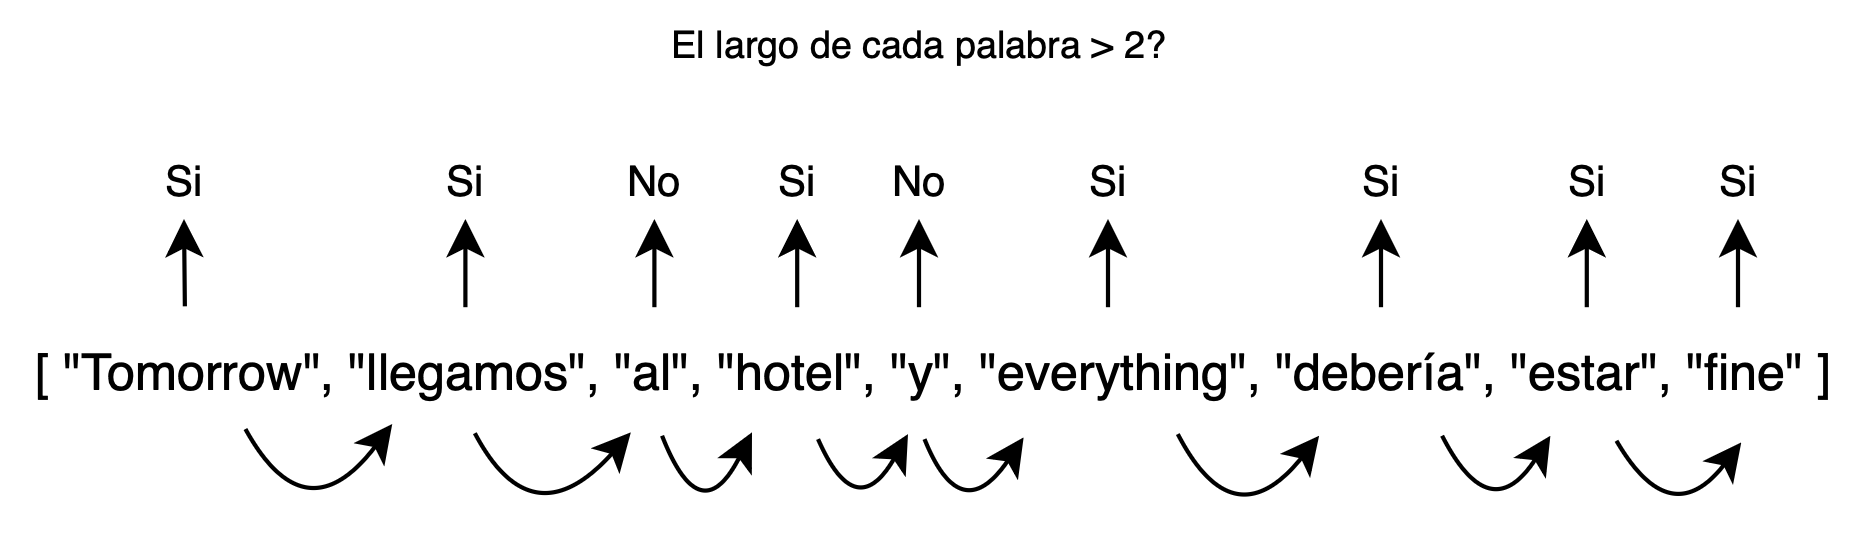
\includegraphics[width=\textwidth]{assets/Reconocimiento_de_lenguaje_P1.png}
    \caption{Reconocimiento de Lenguaje, oración inicial}
    \label{fig:Reconocimiento de Lenguaje P1}
\end{figure}

Una vez se han identificado las palabras "ancla", se procede a identificar la probabilidad de idioma en cada palabra seleccionada, como se puede ver en la figura \ref{fig:Reconocimiento de Lenguaje P2}, tenemos palabras donde la probabilidad de idioma es muy alta, como por ejemplo "Tomorrow" donde su probabilidad de inglés es de un 97.3\% y "debería" donde la probabilidad de español es del 100\%, pero en cambio tenemos palabras como "hotel" que con sus probabilidades de inglés de un 33.6\% (siendo esta la más predominante) y español en un 32.3\%, lo que genera un estado de inconsistencia o estado indeterminado, por lo que en vez de escoger directamente el idioma con la probabilidad más alta directamente, procederemos a calcular el error absoluto entre las probabilidades de cada idioma con:

\begin{math}
\displaystyle \left| P(\text{Idioma\_1}) - P(\text{Idioma\_2}) \right| \geq 0.25
\end{math}

\begin{figure}[H]
    \centering
    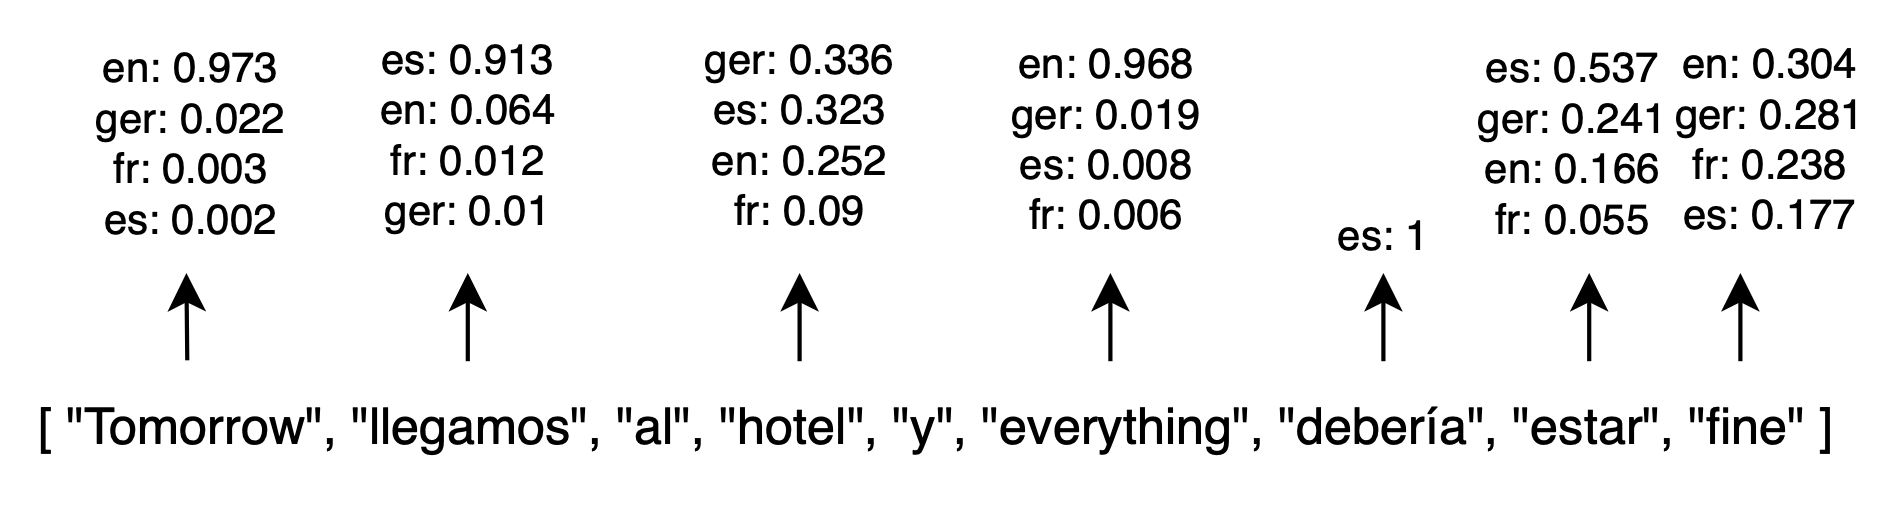
\includegraphics[width=\textwidth]{assets/Reconocimiento_de_lenguaje_P2.png}
    \caption{Reconocimiento de Lenguaje, palabra ambigua}
    \label{fig:Reconocimiento de Lenguaje P2}
\end{figure}

En el caso de que esta diferencia sea menor a 0.25, se considera que la palabra es ambigua y se procede a generar un contexto para esta palabra con el fin de determinar el idioma predominante en ese contexto (sin olvidar las probabilidades obtenidas previamente), en caso contrario a esta palabra se le asigna el idioma con la probabilidad más alta.

\begin{figure}[H]
    \centering
    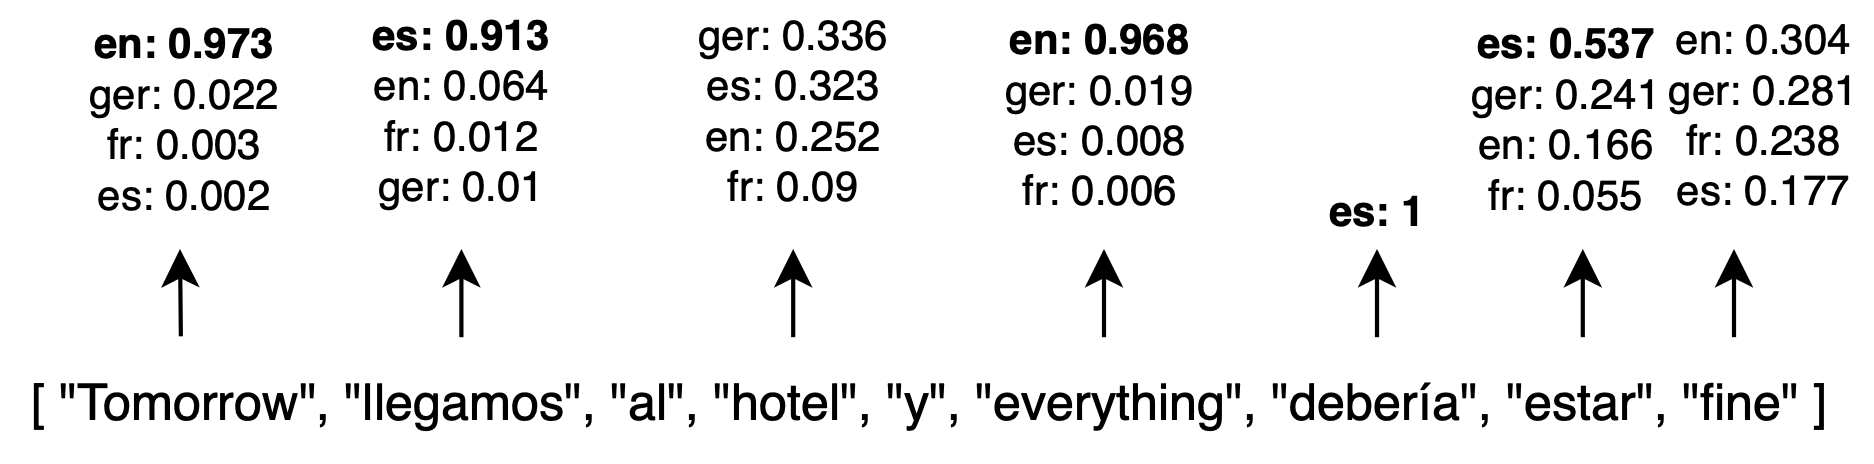
\includegraphics[width=\textwidth]{assets/Reconocimiento_de_lenguaje_P3.1.png}
    \caption{Reconocimiento de Lenguaje, ventana de contexto}
    \label{fig:Reconocimiento de Lenguaje P3}
\end{figure}

Una vez tenemos identificado el idioma de cada una de las palabras "anclas", tenemos que proceder a identificar el idioma de las palabras ambiguas, para esto se genera una ventana de contexto variable (para este ejemplo se usará una ventana de 2 palabras y para nuestra investigación se aplicó un contexto de 3 palabras) alrededor de la palabra ambigua, con esta ventana se llevará a cabo un calculo de peso para cada palabra excluyendo la palabra ambigua, en donde se considerará la probabilidad de idioma que obtuvo la palabra "ancla" adyacente y adicionalmente la posición que tiene esta dentro del texto, con el fin de determinar el idioma predominante en esta ventana de contexto y así asignar el idioma a la palabra ambigua.

La formula de peso de la palabra vecina destinada para este proceso es la siguiente:

\begin{math}
\displaystyle W_{neighbor} = P(neighbor)_{best}^{2} \times \left(\frac{1}{|pos_{neighbor} - pos_{target}|} \right)
\end{math}

Donde $P(neighbor)_{best}$ es la probabilidad más alta obtenida por la palabra vecina para un idioma específico, y $pos_{neighbor}$ y $pos_{target}$ son las posiciones de la palabra vecina y la palabra objetivo (palabra ambigua) respectivamente. Con esta formula se busca asignar un peso mayor a las palabras vecinas que tengan una probabilidad de idioma más alta y que estén más cercanas a la palabra ambigua, con el fin de determinar el idioma predominante en esta ventana de contexto y así asignar el idioma a la palabra ambigua.

Cabe recalcar que en el caso de que una de las palabras del contexto haya sido descartada por tener una cantidad de caracteres menor a 3 caracteres, esta no será considerada para el calculo de peso, ya que como se mencionó anteriormente, estas pueden generar ruido en la detección de idiomas.

Como se puede ver en la figura \ref{fig:Reconocimiento de Lenguaje P4}, tenemos una palabra ambigua "hotel" que se encuentra entre dos palabras "ancla" con probabilidades de idioma muy altas, por lo que se procede a calcular el peso de cada una de estas palabras vecinas para determinar el idioma predominante en esta ventana de contexto, qudando la palabra "llegamos" con un peso de 0.416 y la palabra "everything" con un peso de 0.468, por lo que al tener un peso muy parecido, esta palabra se mantine como ambigua y se deberá considerar un último criterio.

\begin{figure}[H]
    \centering
    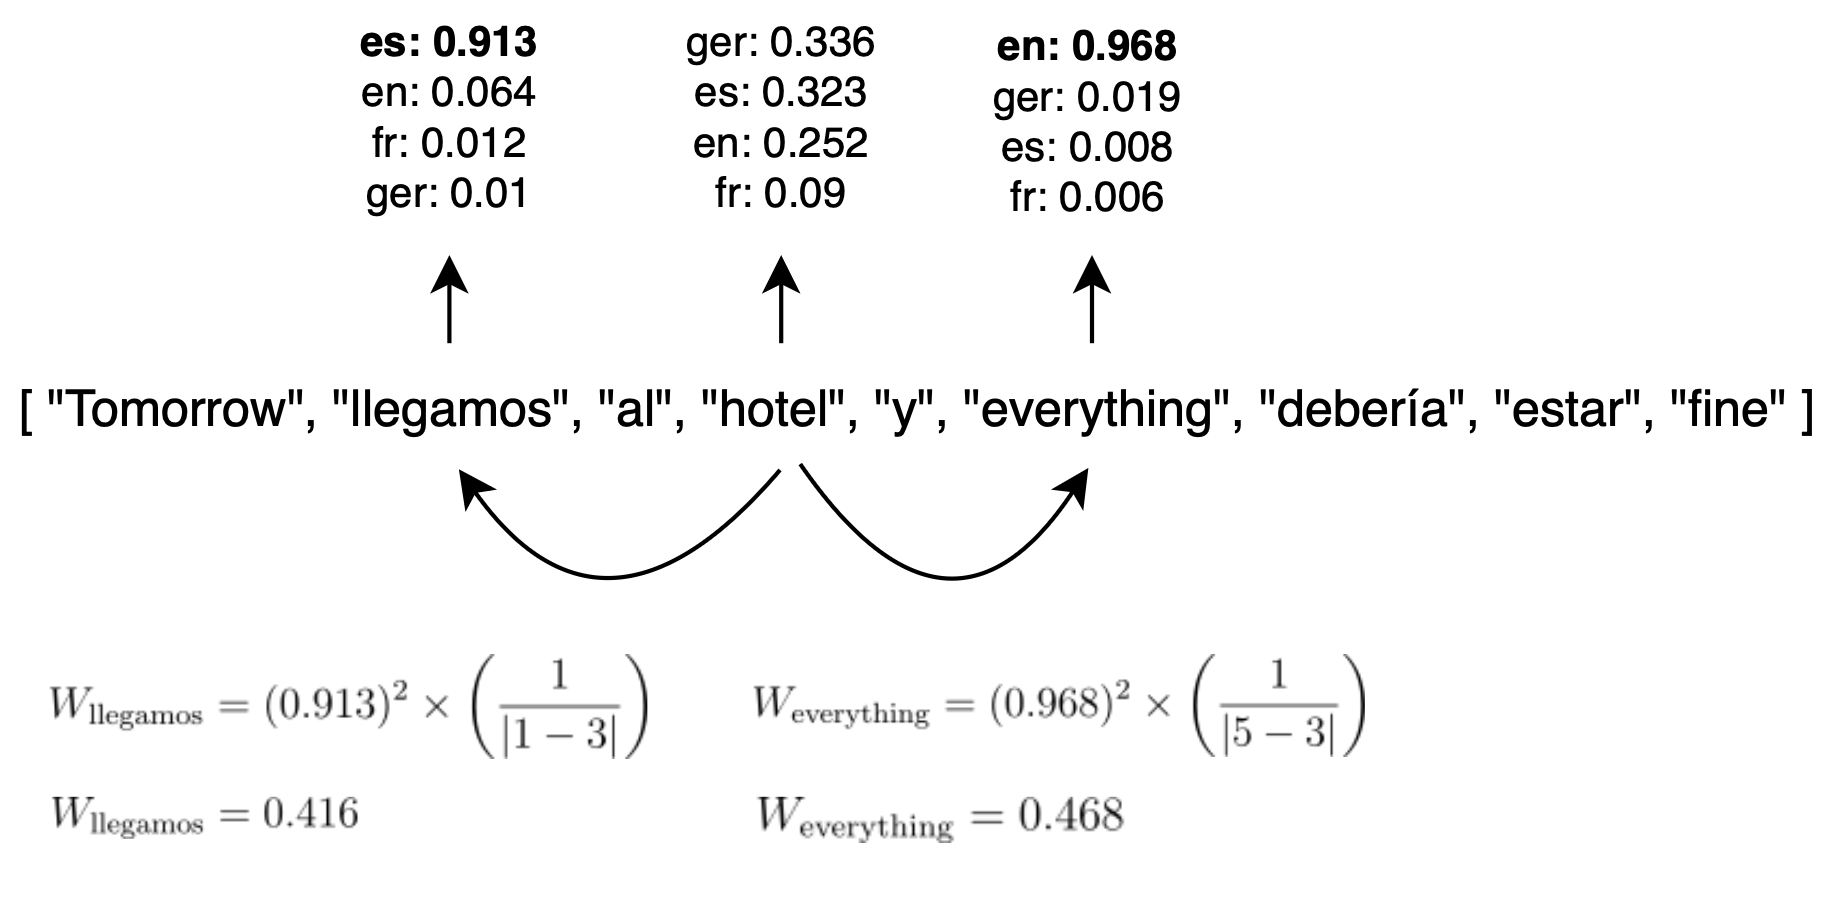
\includegraphics[width=\textwidth]{assets/Reconocimiento_de_lenguaje_P3.2.png}
    \caption{Reconocimiento de Lenguaje, idioma reconocido por contexto}
    \label{fig:Reconocimiento de Lenguaje P4}
\end{figure}

Para este punto en donde tenemos una palabra ambigua con pesos muy similares en su contexto, se procederá a aumentar la probabilidad del mismo idioma que tenga esta palabra en comparación con el idioma detectado globalmente, con el fin de favorecer el idioma que tenga una mayor probabilidad global en el comentario, lo que nos ayudará a determinar el idioma predominante en esta ventana de contexto y así asignar el idioma a la palabra ambigua, por ejemplo en nuestro ejemplo procederemos a darle un peso adicional al idioma español +0.8 lo cuál termina quedando una competecia del español con 0.416 + 0.8 = 1.216 vs en inglés con 0.468, quedando finalmente esta palabra como parte del idioma español, lo que nos ayuda a mejorar la precisión de la detección de idiomas en nuestro dataset y así obtener una mejor aproximación del idioma predominante en cada comentario.

\subsection{\textbf{Detección 3: Agregación por Mayoría Estadística}}
\label{cha:Aggregation by Statistical Majority}

Una vez se ha identificado el idioma de cada una de las palabras presentes en el comentario, se procede a realizar un segundo proceso de selección por idioma predominante, el cúal consiste en sumar las probabilidades del idioma predominante de cada una de las palabras consideradas "anclas" para el comentario y luego dividir esta suma por la suma total de probabilidades de todas las palabras "anclas" para obtener un porcentaje de predominancia del idioma en el comentario, lo que nos ayudará a determinar si realmente el idioma detectado es predominante en base a su mayoría estadística.

La formula que se utiliza para este proceso es la siguiente:

\begin{math}
\displaystyle \text{Majority\_Percentage} = \frac{\sum P(lang_{best})}{\sum P(all\_langs)}
\end{math}

Donde $\sum P(lang_{best})$ es la suma de las probabilidades del idioma predominante de cada una de las palabras "anclas" para el comentario, y $\sum P(all\_langs)$ es la suma total de probabilidades de todos los idomas de todas las palabras "anclas" para el comentario. Con esta formula se busca obtener un porcentaje de predominancia del idioma, lo que nos ayudará a determinar si realmente el idioma detectado es predominante en base a su mayoría estadística, y así mejorar la precisión de la detección de idiomas en nuestro dataset.

% insertar figura de ejemplo de reconocimiento de lenguaje
\section{\textbf{Eliminación de columnas}}
Se eliminan las columnas innecesarias del dataset, conservando solo aquellas relevantes para el posterior análisis. En nuestro caso, estas columnas son: \textbf{title}, \textbf{review\_text} y \textbf{language}, ya que estas contienen la información relevante para el análisis de sugerencias, mientras que las demás columnas pueden generar ruido o no aportar información relevante para nuestro objetivo.

\section{\textbf{Filtrado de datos}}
Una vez reconocido el lenguaje de los comentarios continuaremos con el filtrado de idioma de los datos, por lo cuál pasaremos principalmente por dos criteríos, el primero de ellos es que el lenguaje detectado con la fase de detección global de idioma \ref{cha:global_detection_lang} y el detectado por la fase de análisis micro-simántica \ref{cha:micro-semantic analysis} deben coincidir, ya que si estos no coinciden, esto puede generar una inconsistencia en el idioma del comentario, y adicionalmente el valor de majority\_percentage obtenido en la tercera fase \ref{cha:Aggregation by Statistical Majority} debe ser mayor a un 0.5, lo que nos asegura que el idioma predominante en el comentario es realmente predominante en base a su mayoría estadística.

